\chapter*{A Note on Data Dimensionality}

While we aim to demonstrate the application of high dimensionality in these studies, we do not wish to mislead readers that we have assembled a 12-dimensional photometric dataset, simply because we have 12 wavebands. This statement may seem nonsensical at first, but makes sense when we consider the covariance of the data. Just from the outside, and our faithful belief that FIR dust emission looks something like a blackbody, or modified blackbody, or at the very least we can agree that emission from dust in thermal equilibrium would produce some sort of peaked continuum emission spanning multiple photometraic bands' width. If we agree on this point, then it follows naturally that said bands would be highly correlated with one another. This means that the number of truly independent data dimensions is not only lower than the number of bands used here, it is much lower.

Fig. \hyperref[fig:pca_intro]{\ref{fig:pca_intro}} shows the \% of variance in the data retained by the first $n$ principal components. Principal components are found essentially by first finding the covariance matrix of the input data, and then diaganolizing this matrix- the eigenvectors will be the basis vectors of each principal component. The eigenvalues will give the explained covariance per component. Applied in this manner, the components may not necessarily have a clear physical interpretation, but from a data analytics perspective we can at least assess the redundancies in our data. Thus from Fig. \hyperref[fig:pca_intro]{\ref{fig:pca_intro}}, and choosing an arbitrary covariance ``acceptable loss'' of 99\%, our photometric data set steeply reduces to 3 dimensions. The first component contains 98\% of the total variance.


\begin{figure*}
  \label{fig:pca_intro}
  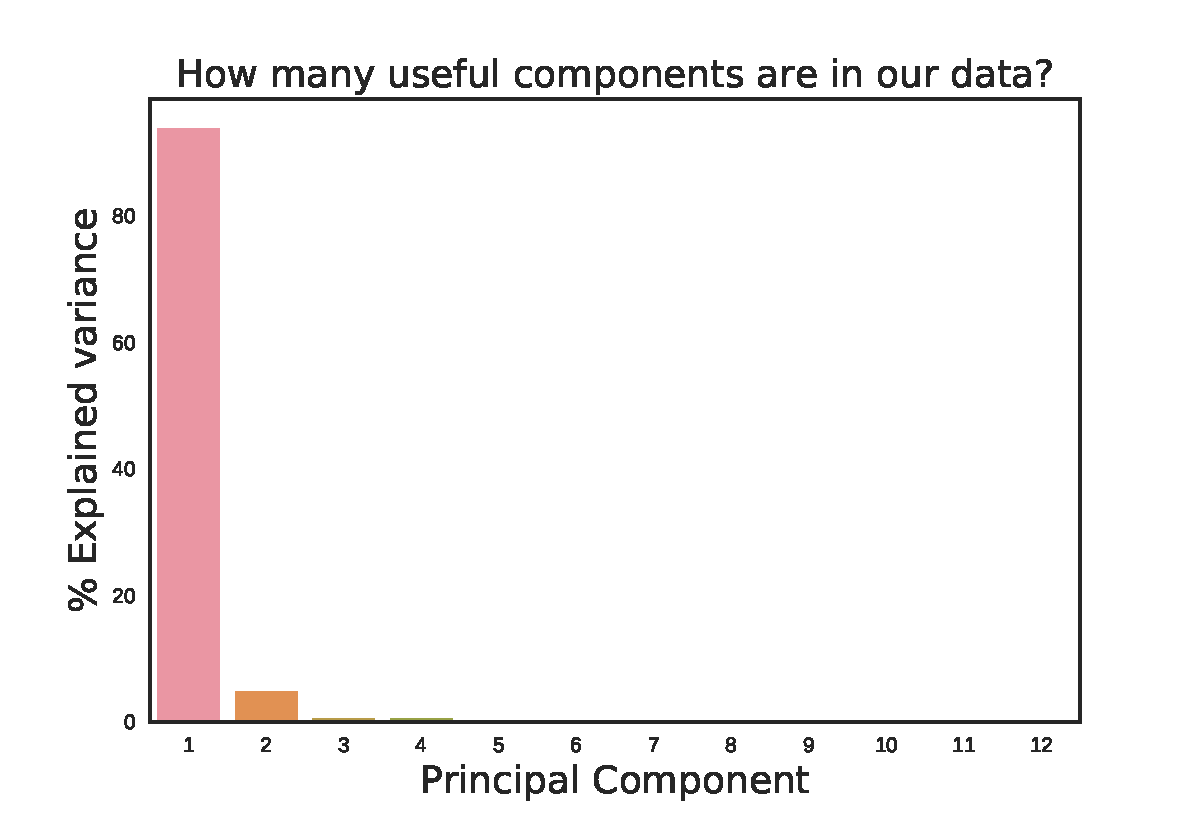
\includegraphics[width=\textwidth]{../Plots/ch_intro/pca_intro.pdf}
  \centering
  \caption{Explained variance decline for principal component analysis performed on a set of 12 all-sky infrared maps. The first three components account for over 99\% of the total variance. The PCA fit is performed on the whole sky, after whitening the data, using the ``scikitlearn }
\end{figure*}
